\begin{refsection}

\chapter[Dynamic function of neurons]{The function of groups of neurons changes from moment to moment}

\section{Abstract}
Modern techniques that enable identification and targeted manipulation of neuron groups are frequently used to bolster theories that attribute specific behavioral functions to specific neuron types. These same techniques can also be used, however, to highlight limitations of such attribution, and to develop the argument that the question ‘what is the function of these neurons?’ is ill-posed in the absence of temporal and network constraints. Here we do this by first reviewing evidence that neural responses are dynamic at multiple time scales, making the point that such changes in firing rates imply changes in what the neuron is doing. Studies involving brief perturbations of neural populations confirm this point, showing that the functions in which these populations participate change across seconds and even milliseconds. Based on these studies, we suggest that it is inappropriate to assign function to sets of neurons without contextualizing that assignment to specific times and network conditions.

\section{Introduction}
The increasing availability of sophisticated molecular biological techniques affords neuroscientists new means of interrogating the function of specific neurons and neuron groups. It has become commonplace to track the identity of neurons that are active as an animal performs a behavior, and to silence genetically identified (or pathway-specific) sets of neurons in the context of recording/imaging/behavioral experiments. The nature of these techniques is such that when experimenters make performance worse by silencing a set of neurons, the experimenters inevitably conclude that they have uncovered the function (or at least a function) of that set of neurons; null results are interpreted as evidence that the neurons responsible for that function have yet to be isolated. The development and use of these techniques synergizes with the popularity of theories in which function is ascribed to identifiable cell groups, both testing and driving such theories.

This approach has been remarkably successful, in that the recent literature is rife with articles enumerating the involvement of specific cell types in specific neural or behavioral functions (\cite{adamantidis2015a,balthazart2020a,biselli2019a,janak2015a,tye2012a}). It is worth noting, however, that while these modern techniques allow the experimenter to directly assay or manipulate the firing of a single cell type, observing a significant decrement in some behavioral measure as a result of silencing one set of neurons does not necessarily imply that the set of neurons in question is uniquely involved in the function under study. As just one general example, results showing that silencing projection neurons has one effect whereas silencing inhibitory interneurons has the opposite effect may not imply different specific functions for those two neuron types, but rather a wholistic function of a network of interconnected neurons that is perturbed in opposite directions by manipulations that impact overall network excitability in opposing ways.

But the fecundity of neural interconnections does not just mean that function within circuits is almost necessarily distributed among multiple cell types. These interconnections also motivate an argument that the entire research endeavor should be reconsidered — that the very act of mapping function (or at least behavioral function) onto cell types ignores the complex dynamics of neural ensemble responses, and that ascribing specific functions to specific neurons is unwarranted. This is the argument that we unpack here: we start with evidence that the multi-scale firing dynamics — firing-rate dynamics that are part and parcel of the activity of neurons embedded within networks — means that function changes across learning, across changes in context, and even across parts of seconds. We go on to show that the impact of perturbing the activity of neural ensembles differs depending on the timing of the disruption, and that even two identically timed perturbations may have different impacts (because firing-rate dynamics do not necessarily unfold at the same rates in all trials). These data reveal that the functions of neurons can change dramatically over even very short spans of time, and motivate our conclusion that function is only properly assigned to groups of neurons when those neurons are placed in specific times and specific network conditions.

\section{Forebrain neural activity is intrinsically dynamic}
Most theories that ascribe particular functions to specific neurons use single numbers — average firing-rate magnitudes — to characterize those neurons’ responses. Neurons are classically said to ‘code’ a sensory stimulus if the average number of spikes that they fire (across a reasonable interval) in response to that stimulus significantly exceeds their spontaneous firing rate; each neuron is simply characterized as either responding significantly or not, or as having fired more or less than to other stimuli (analogous arguments can be made regarding activity related to movement, of course). Thus, it makes sense to conceptualize that neuron’s involvement in processing the stimulus in an equally simple way (\cite{chen2011a,hubel1995a,lavi2018a,mazurek2014a,steinmetz2019a,wang2018a}) — for example, saying that a neuron that responds to sucrose, or that responds more to sucrose than to other tastes, functions to code sucrose.

If function can be attributed to a neuron on the basis of response magnitude, however, then by the same logic, changes in function can be attributed to changes in response magnitudes — a fact that complicates attempts at simple conceptualizations of function. The truth of this logic is visible in studies of learning in the brain, and more specifically in the common (if seldom explicitly articulated) recognition that learning-related changes in neural firing represent the assumption of a new function by that neuron (that of driving learned behavior [\cite{banerjee2020a,barsy2020a,ross2018a}]). For just one classic example, consider a deep cerebellar nucleus neuron that has become responsive to a tone in a conditioned eye blink learning experiment; this neuron can be said to have acquired the function of driving an eyeblink (\cite{mm2017a}).

More recent examples make use of the very same molecular/genetic techniques that have reinforced simple theorizing about the function of neuron groups (\cite{aqrabawi2020a,butler2020a,josselyn2018a,josselyn2020a,sun2020a}). Notable among this recent work are studies showing that activation of a group of context-responsive hippocampal dentate gyrus neurons causes mice to freeze (presumably in fright) after successful fear conditioning; before the completion of conditioning, activation of these neurons does not induce freezing (\cite{ramirez2013a}). Analogously, extinguishing the prior-acquired fear memory also changes the response properties of a specific set of neurons in amygdala. Reactivation of these ‘extinction-responding’ cells comes to facilitate fear extinction behavior following learning, but does not do so before (\cite{zhang2020a}). These results drive home the point that when learning-relevant experiences change the responses of small groups of neurons, the functions in which these neurons participate change (e.g., come to drive or antagonize fear response).

But neural responses are not only plastic with learning. A growing body of evidence attests to the fact that neural responses can readily shift with changes in experimental context — that recent experience and the understanding of the regularities of the stimulus environment (non-randomness of what stimuli appear and when) can modulate the specific properties of neural and behavioral responses to input stimuli (\cite{flores2018a,noudoost2017a}), as can the current state of the networks into which the neurons are embedded (\cite{sakata2016a}) or connected (\cite{mante2013a,safaai2015a}). Furthermore, a sensory neuron’s response may mean different things to downstream neurons in different contexts: in drosophila, for instance, the responses of looming-responsive neurons (neurons that respond to visual stimulus expansion) have distinct implications depending upon the fly’s flight status; activation of these neurons during flight instigates landing behavior, whereas activation with visual stimuli while ‘grounded’ activates different motor programs (\cite{ache2019a}). Note that while the function to which these neurons’ activity contributes depends on the stimulus (and activity driven by said stimulus), it depends with equal importance on the animal’s current state; context alters both the sensory neuron’s response and the use of that neuron’s response. This result is echoed in recent work demonstrating that the central circuit involved in processing olfactory input depends on behavioral context: taste cortex has proven to be integrally involved in olfaction, but only when the rodent is feeding, not when it is inhaling (\cite{blankenship2019a}).

The above work reveals that neurons’ responses following stimulus presentation (or, for that matter, before behavior) may change according to variables that themselves change on sub second time scales. An implication is that neural responses may undergo significant and meaningful changes across very short time periods. Recent evidence confirms this, demonstrating that single neural responses may actually be made up of multiple distinct firing rate ‘epochs’, with sequences of firing-rate changes unfolding across tens to hundreds of milliseconds (\cite{guo2015a,sauerbrei2020a,sugase1999a}). A relevant example comes from work on gustatory (taste) coding, which has this dynamic property at most central relays (\cite{baez-santiago2016a,fontanini2008a,li2016a,li2013a}): cortical single-neuron taste responses, for instance, actually involve three firing-rate epochs, each of which contains distinct information content; the initial response contains little taste-related information, the second epoch provides a firing-rate code for which taste is on the tongue, and the third epoch contains firing that is correlated with taste palatability (and therefore the animal’s decision whether to consume). The onset latency of this last epoch varies widely from trial to trial, but consistently predicts the onset of consumption behaviors (\cite{sadacca2012a}).

Actually, such firing rate dynamics are an almost inevitable facet of activity in complex interconnected networks (\cite{pandarinath2018a,yuste2015a}) — feedback causes neurons to be repeatedly ‘re-modulated’ by new sources of input, for example, as activity first percolates through a region via asending pathways and then again via feedback pathways. Given this fact, it is unsurprising that such dynamics are frequently observed. As explained above, their occurrence calls researchers’ tendency to ascribe general functions to specific neurons into question — by the same logic described with regard to learning-related changes, these changes in firing rates represent evidence that the nature(s) of the function(s) in which these neurons are involved also change across even very short spans of time.

\section{Perturbation studies confirm the ‘dynamics’ of neuron function}
Of course, the above evidence is largely phenomenological: firing rate dynamics suggest dynamics of function, but do not prove them; even studies in which firing rate changes are rigorously controlled by the experimenter (i.e. induced by optogenetic activation) are non-conclusive, because their interpretation relies on the questionable assumption that optogenetic firing-rate enhancements of a set of neurons is analogous to natural firing-rate changes. More compelling evidence would come from studies in which brief perturbations, designed not to mimic the natural situation but to disrupt it, are shown to have (or not to have) differing impacts depending on whether they are timed to disrupt firing at one particular time or another.

It is only recently that such experiments have become feasible, and thus few have as of yet been done, but the results have been striking. When, for instance, rodent sensorimotor cortex is optogenetically suppressed before or during a complex reach (a behavior that involves highly dynamic neural activity in this region), the impact of that suppression depends both on context — whether the movement is trained or naïve — and the perturbation’s precise timing (\cite{guo2015a}) (Figure 1). Perturbations delivered just before execution of the trained movement halt grasping completely, for instance, whereas the same is not true of the naïve reach. Furthermore, when the perturbations are delivered only (tens to hundreds of milliseconds) after trained reaches are initiated, these perturbations only halt movement after the current stage of the movement reached completion and even later perturbation onsets often fail to inhibit movement at all, allowing the animal to successfully retrieve food. Thus, sensorimotor cortex is differentially involved in the initiation and early aspects of trained movement.

\begin{figure}
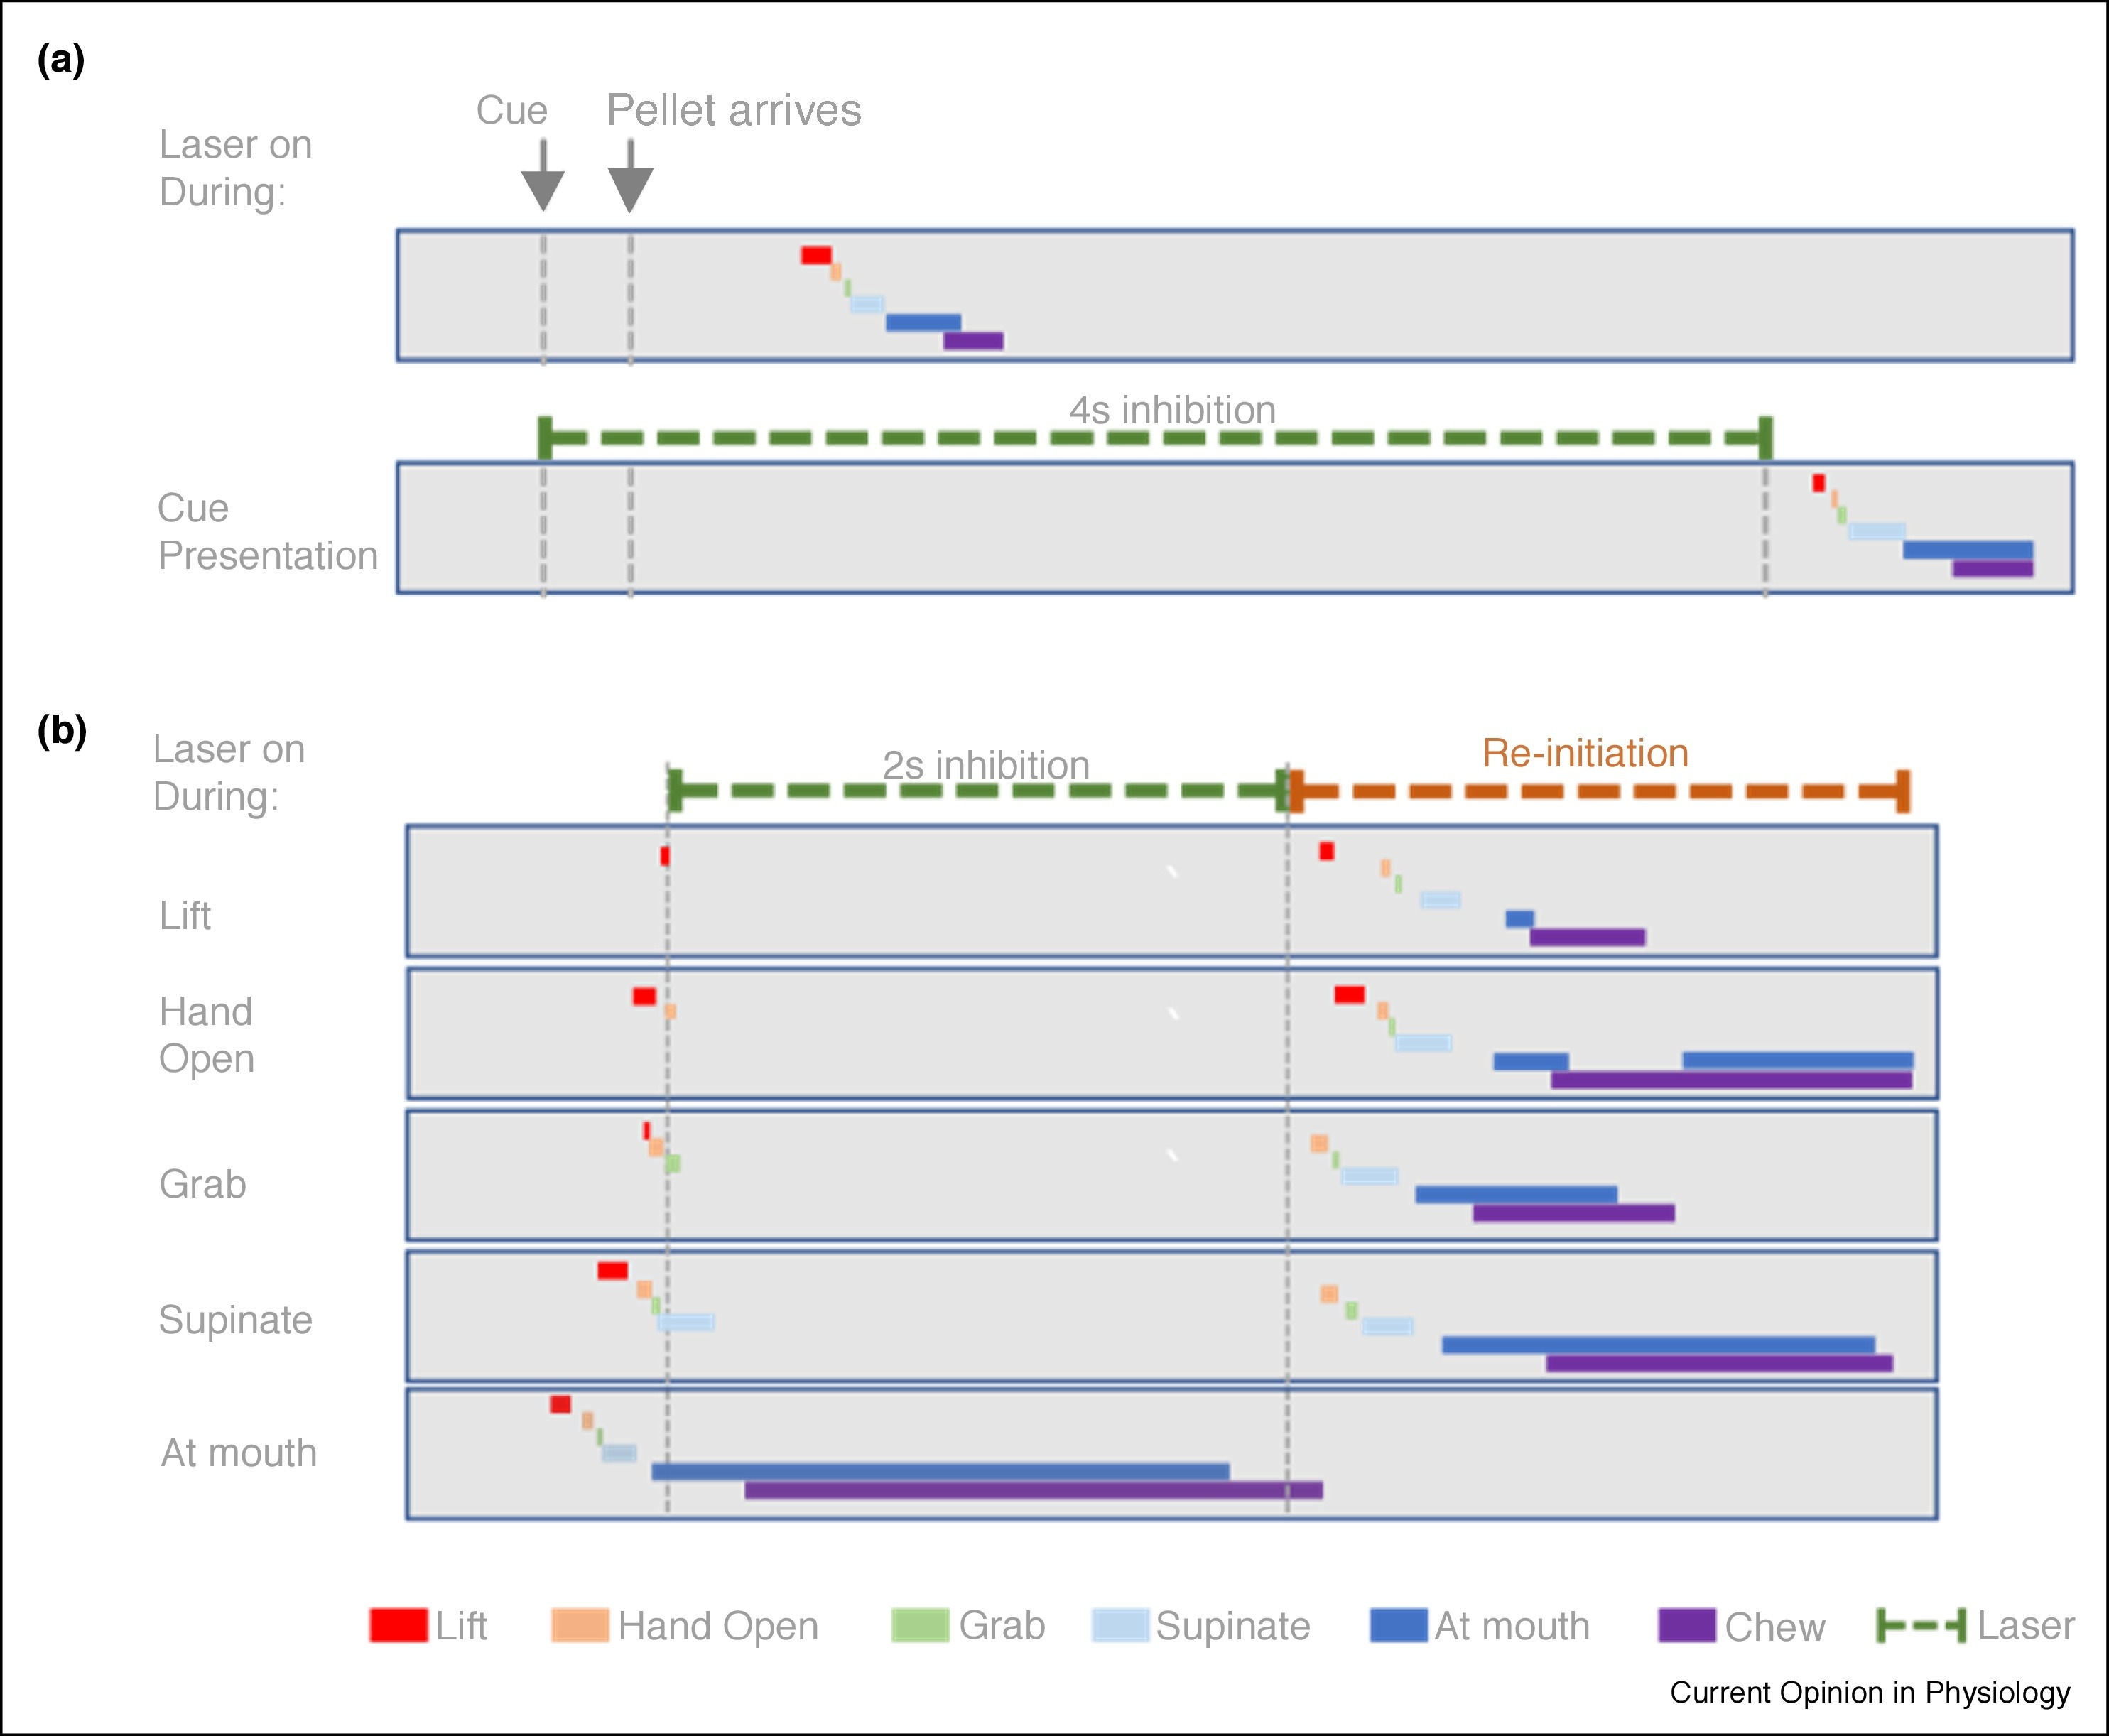
\includegraphics[width=\linewidth]{lin_2021_review_figs/1-s2.0-S2468867320301693-gr1_lrg.jpg}
\caption{\textbf{Dynamic involvement of sensorimotor cortex in well-trained grasping behavior.} \textbf{(a)} Representative trials of multi-stage grasping behavior during control trials (top panel) and sensorimotor cortex inhibition trials (bottom panel). Following the tone-cue presentation, a food pellet was delivered in front of a head-fixed mouse, which would then initiate a grasping movement involving a (∼700 msec) sequence of six sub movements: lift, paw open, grab, supinate, at mouth, and chew. The entire sequence was prevented when the sensorimotor cortex was inhibited optogenetically (indicated by green dashed line) via stimulation of GABAergic inhibitory neurons. The behavior was reinitiated once the laser was turned off. \textbf{(b)} Representative trials in which inhibition was induced at different time-points in the movement. The impact of post-onset perturbations was not immediate, but rather emerged after a delay during which the behavior continued to the beginning of the next component. Cortical perturbations had no impact on impeding hand movement involved in chewing (i.e. at mouth). Note that these are example trials. Durations of some behavioral components are seemingly stretched when sensorimotor cortex was suppressed after behavior being initiated (b), the difference, however, is not statistically significant when all trials were pooled together (cf. Figure 4 of \cite{guo2015a}). The length of color-coded bars denotes the duration of each behavioral component. Figure was adapted from \cite{guo2015a}.}
\label{fig:wrapfig}
\end{figure}



Similarly, the impact of perturbing basolateral amygdalar (BLA) input to the nucleus accumbens (NAcc) in rats trained to make choices between smaller, certain rewards and larger, uncertain rewards (\cite{bercovici2018a}) depends on that perturbation’s specific timing. During trials in which it was applied before animals committed to a choice, the perturbation generally reduced the strength of the rats’ preferences for whichever reward was ‘best’ (i.e. the most rewarding over the long term), regardless of which reward that was (the experimenters were able to change experimental parameters such that the best choice would switch from being the small to the large, or vice versa). If, on the other hand, the BLA→NAcc pathway was inhibited only after uncertain choices that resulted in a lack of reward, the impact was both different and asymmetrical — the perturbation increased the likelihood of risky choices in subsequent trials (Figure 2). The BLA→NAcc connection appears to have different functions at different moments in the task.

\begin{figure}
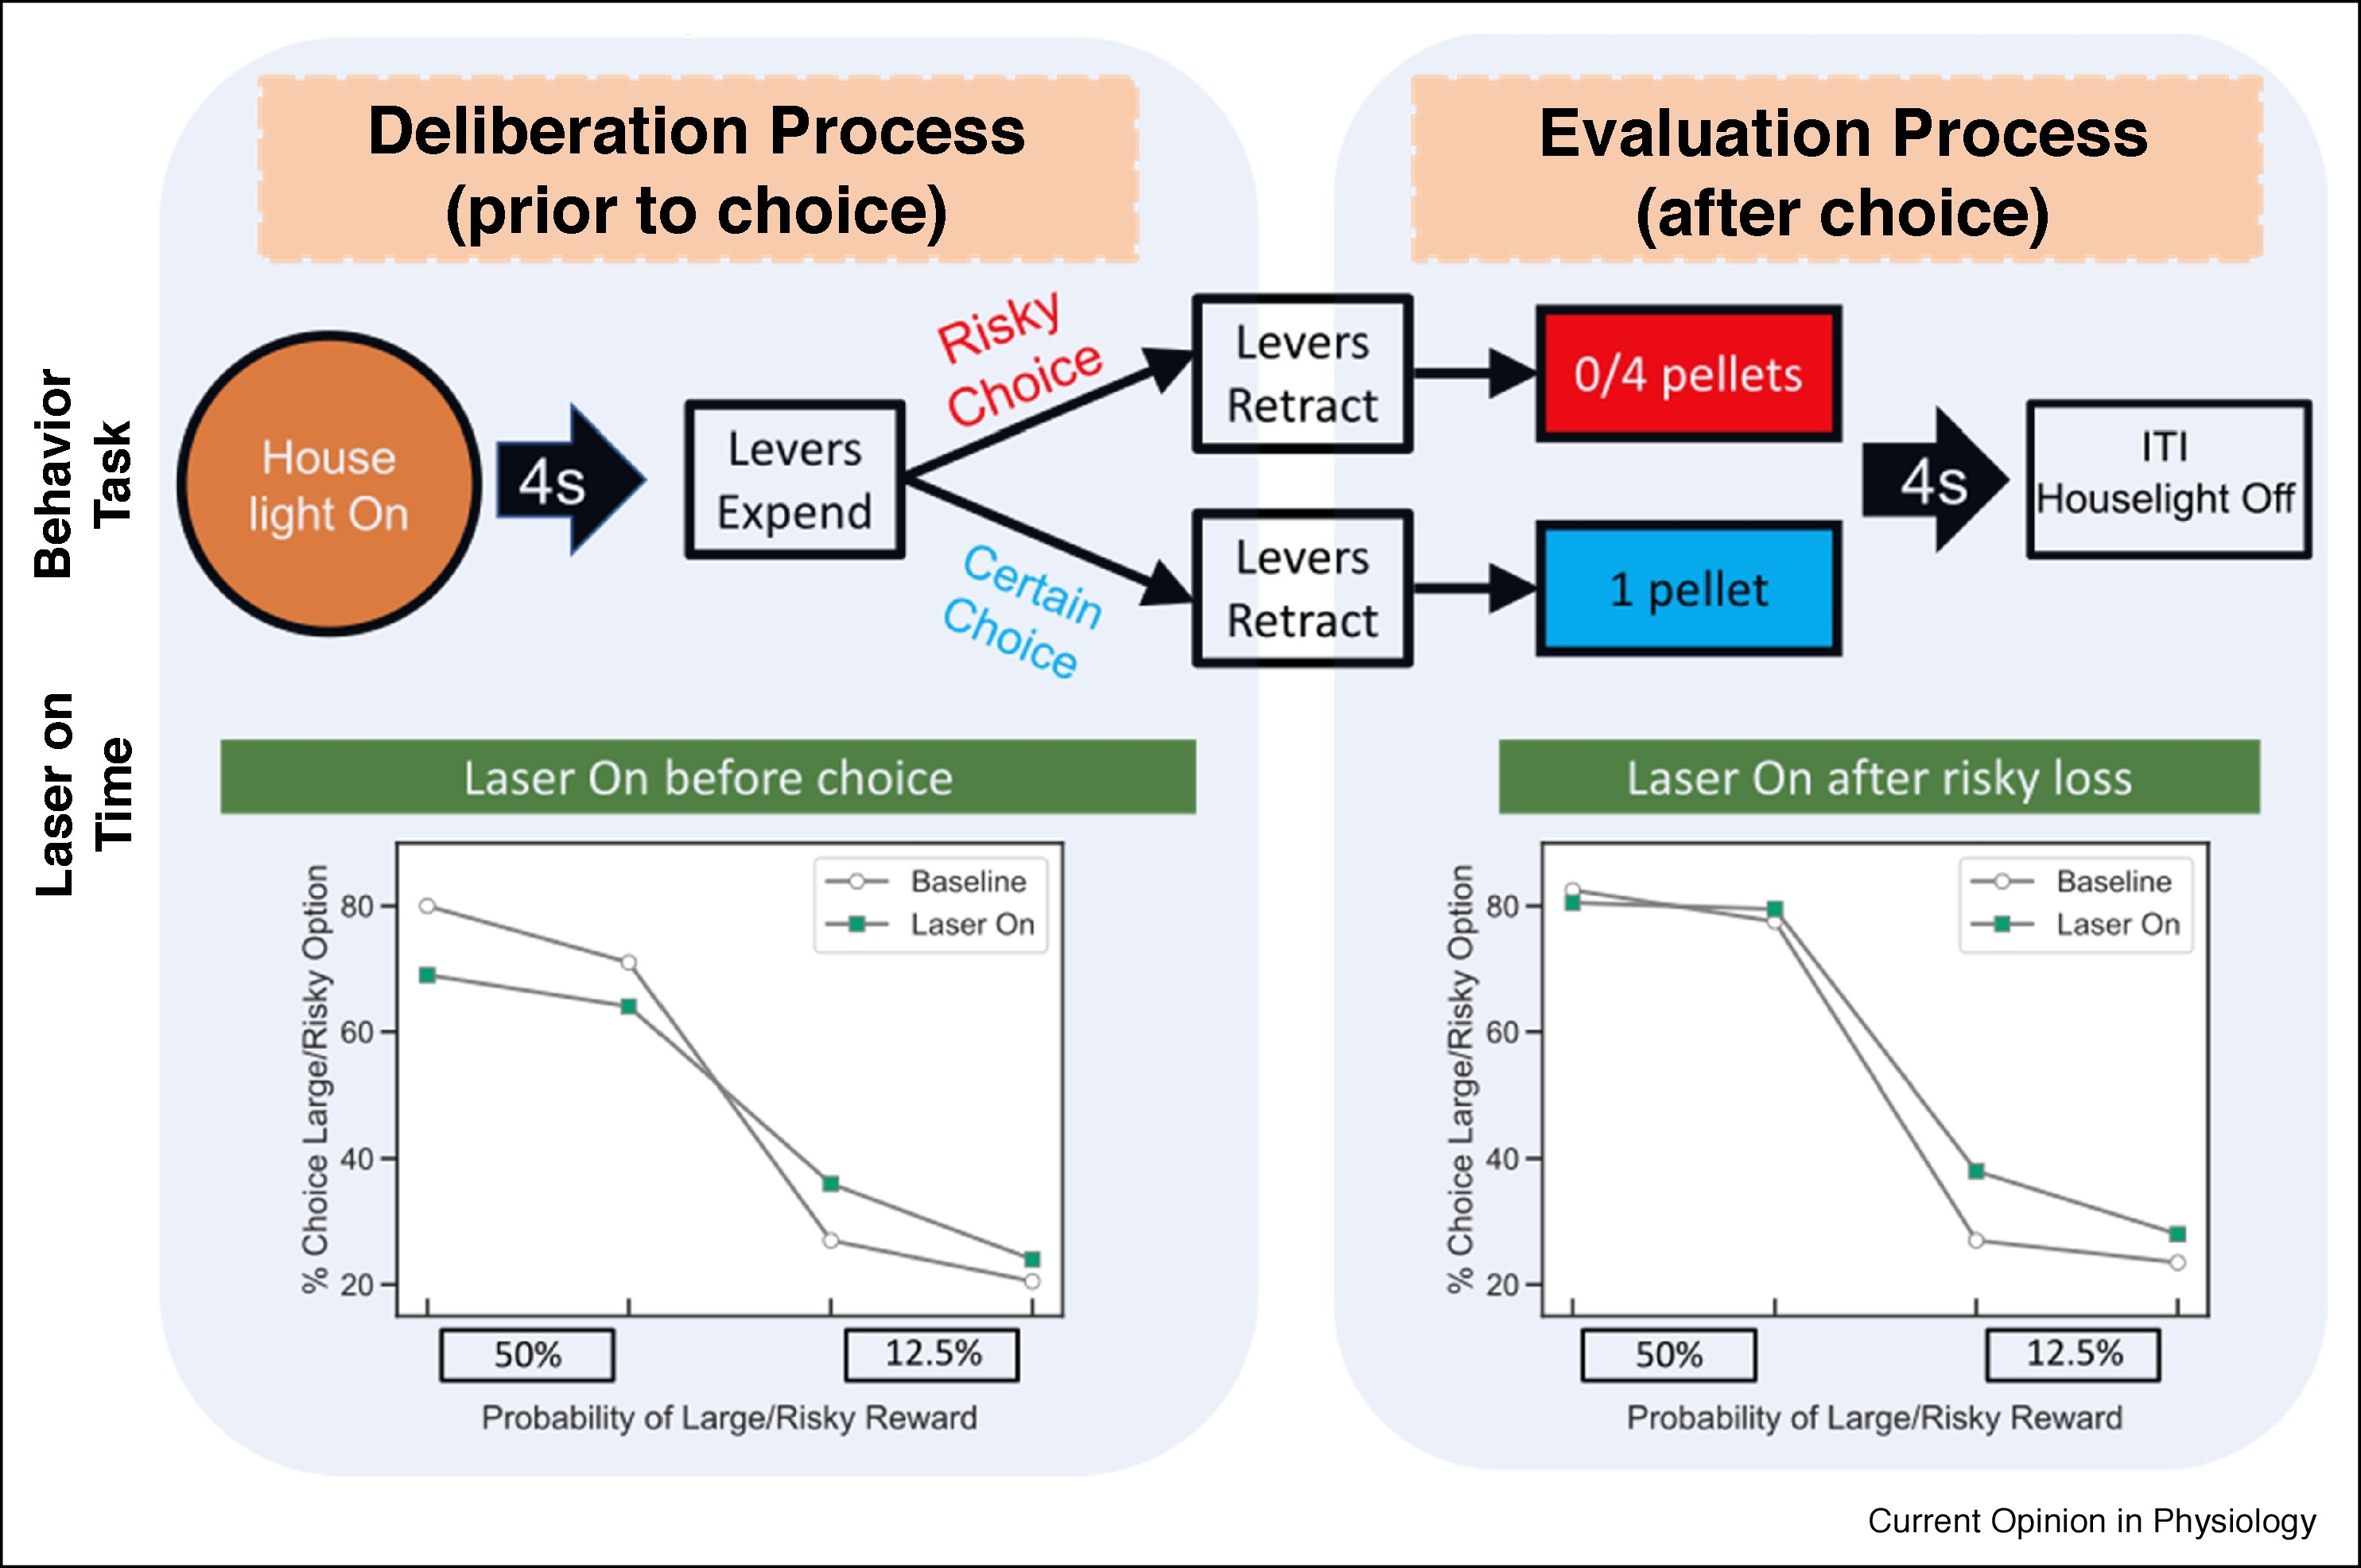
\includegraphics[width=\linewidth]{lin_2021_review_figs/1-s2.0-S2468867320301693-gr2_lrg.jpg}
\caption{\textbf{Functional dynamics of basolateral amygdala (BLA)→nucleus accumbens (NAcc) projection during a decision-making process.} The BLA→NAcc circuitry is involved in decision-making when reward is uncertain. Following acquisition of a probabilistic discounting task, rats received optogenetic inhibition of BLA→NAcc axons (as those axons enter NAcc) either before the choice (during the deliberation process) or after (during the evaluation of choice). The former inhibition significantly reduced subsequent preferences for the optimal choice — decreasing the likelihood of a risky choice when reward probability was 50\% but decreasing the probability of a safe choice when reward probability was lower (12.5\%). If, meanwhile, BLA→NAcc was inhibited after a choice that led to reward omission, the likelihood of selecting the risky choice increased, but only during the low probability (12.5\%) block. ITI: inter-trial interval. Figure was adapted from Bercovici et al. (\cite{bercovici2018a}).}
\label{fig:wrapfig}
\end{figure}

Of course, in each of the above paradigms, observed firing rates dynamics occur in concert with changes in outward behaviors. To some degree, therefore, it is unsurprising that perturbations of firing at different moments are associated with different changes in specific function, because the animals are doing (at least slightly) different things at different moments. The most risky tests of our thesis (the argument that the function being performed by specific groups of neurons changes across even short stretches of time) will therefore involve neural dynamics that occur in the absence of such outward behavioral dynamics, such as the afore-mentioned cortical coding sequence that spans the gap between the moment that a taste hits the tongue and the moment that discriminative consumption behaviors (ejecting or swallowing) occur.

We have performed this test, taking advantage of the fact that neural ensemble analyses reveal that the transitions between these epochs, and in particular the transition into palatability-related firing (\cite{sadacca2016a}), are sudden and clearly discernible in single trials (c.f. (\cite{jones2007a})). The impact of brief (0.5 s) optogenetic inhibition of these neurons has recently been shown to depend exquisitely on the timing of that inhibition: if it begins before the ensemble transition into the palatability state, consumption-related behaviors are greatly delayed; the same perturbation delivered even just a few tens of msec after the transition, however, has no impact on behavior (\cite{mukherjee2019a}) (Figure 3). Given the fact that palatability-related firing emerges at different times on different trials, two outwardly identical perturbations (i.e. both occurring at 700 ms after taste delivery) will have predictably different impacts depending on whether neurons have reached the point of coding palatability already on that particular trial. The question of what these neurons do is simply ill-posed — their function is only defined with reference to a certain time interval and certain pre-existing conditions in the network.

\begin{figure}
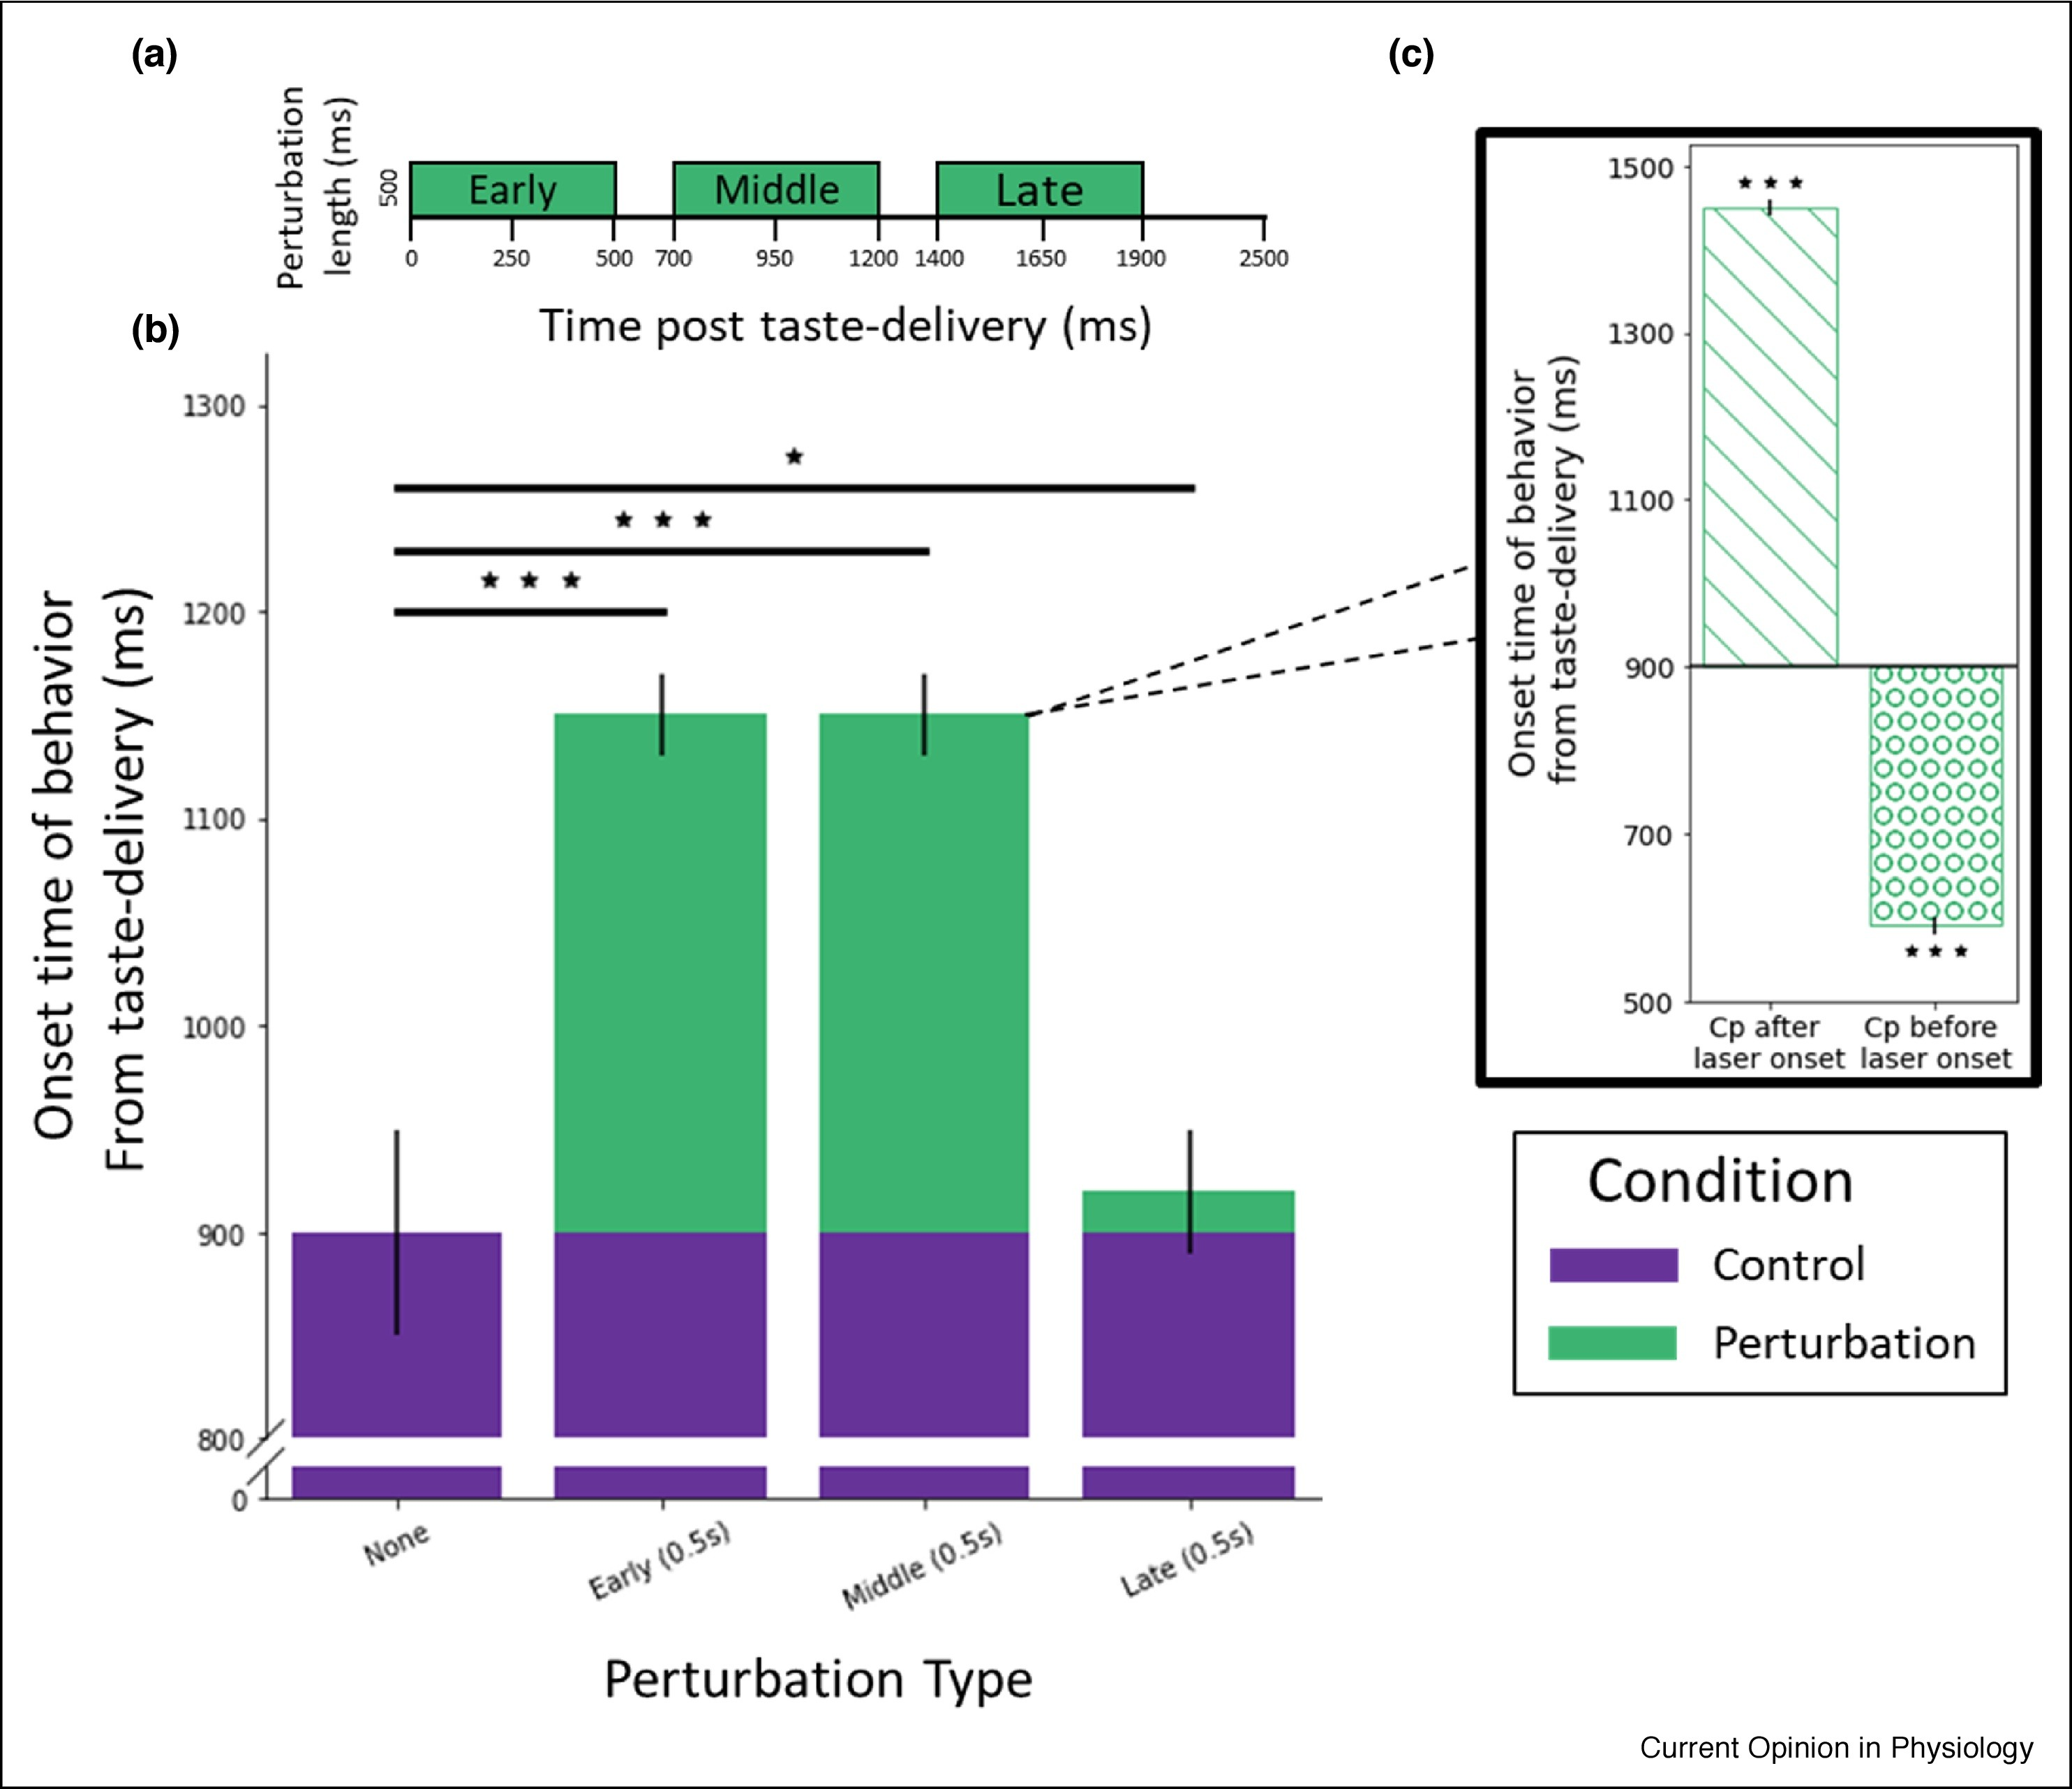
\includegraphics[width=\linewidth]{lin_2021_review_figs/1-s2.0-S2468867320301693-gr3_lrg.jpg}
\caption{\textbf{Behavioral disruption is dependent on precisely timed optogenetic perturbation in gustatory cortex.} (a) Brief (0.5 s) optogenetic inhibition of gustatory cortex was delivered at one of three possible time points post taste-delivery: early (0–0.5 s), middle (0.7–1.2 s), and late (1.4–1.9 s). (b) The bar graph shows the impact (green) of perturbations on latency (y-axis) of gaping (an oral behavior signaling reaching of a rejection decision) to quinine. Purple is the within-session control latency (i.e. on trials with no perturbation). The error bars are the 95\% Bayesian credible intervals (* = p < 0.05, *** = p < 0.001). Early and Middle perturbations of cortical taste responses delayed the onset of gaping, while Late perturbations produce only a minor delay in gaping onset. (c) The apparent impact of Middle perturbation on the onset of aversive orofacial behavior shown in (b) is a mix of actual effects, as the true impact depends exquisitely on the state of the ensemble dynamics just before perturbation onset time in that particular trial. The left bar shows the result of the perturbation during trials in which the palatability-related ensemble transition had not occurred before the time of perturbation onset; the right bar represents trials in which palatability-related firing had already occurred before (in some cases, as little as 20 s before) the laser was switched on (i.e, before 0.65 s; adapted from Mukherjee et al. (\cite{mukherjee2019a})).}
\label{fig:wrapfig}
\end{figure}

\section{Conclusion}
Studies in which neural responses are quantified only in terms of their average firing rate inevitably under describe the complexity of the activity of neurons embedded in networks. Furthermore, it has long been understood that experiments showing that lesion/inactivation/perturbation of a particular set of neurons impacts behavior fall far short of demonstrating those neurons to be the primary locus of that particular behavior. Neurons that are embedded in interacting networks – networks which ensure multi-responsivity and temporal coding – will also demonstrate exquisite sensitivity to changes imposed upon these networks by any of a number of natural internal or external perturbations.

While it is attractive and simple to think of individual neuron groups and types as having distinct and relatively immutable functions, these above considerations make it unlikely that such theories have a great deal of physiological validity. They instead predict function that is distributed and shifting in concert with firing rate changes, and in accordance with dynamical system principles (\cite{jones2006a,camera2019a,miller2016a}). The studies described here confirm these predictions.

\printbibliography[title={References}]

\end{refsection}